\chapter{系统实现}
\section{系统环境搭建}
对于windows系统,要运行本系统,首先需要安装python3,接着下载llvm和clang,然后适当的设置环境变量PYTHONPATH到clang.cindex,或者在py程序中的开头加上

\begin{lstlisting}[language=Python]
clang.cindex.Config.set_library_file(PATH to the libclang.dll)
\end{lstlisting}


然而,在笔者后续的探索中,发现在社区中有人已经替我们做好了这一切,
我们并不需要真的像上述那样在电脑上手动配置环境,如果想使用libclang来获取 C++ 语法树,只需要
\begin{lstlisting}[language=bash]
pip install libclang
\end{lstlisting}
不需要做其他任何操作。
此外,官方提供的包内缺少type hint,若想要比较舒适的开发环境,
可以在\href{https://github.com/16bit-ykiko/clang-related/blob/main/cindex.pyi}{此处}下载相应的提示文件并将它放在与cindex.py同一目录下,
即可获得代码提示。
\section{具体功能实现}
\subsection{从c++源程序到AST}
{\small 
\begin{lstlisting}[language=Python,caption=traverse]
def traverse(node: cx.Cursor, prefix="", is_last=True):
...
    # 分析函数体
    if node.kind is cx.CursorKind.FUNCTION_DECL:
        if node.is_definition():
...

    # 遍历子节点
    for child in children:
        traverse(child, new_prefix, child is children[-1])

\end{lstlisting}
}
该函数首先接受一个cindex.Cursor类型的node作为参数,根据相应的信息打印出AST,这相比于clang自带的AST更加清晰,包含了我们需要的信息,且便于调试。
接着便判断函数的类型是否为FUNCTION\_DECL,如果是,我们还需要判断它是否为函数定义,然后提取该函数定义的函数体,
递归构造自动机,同时维护函数表,将得到的函数名和入口出口保存。
最后,递归调用traverse函数本身。
{\small
\begin{lstlisting}[language=Python,caption=main]
def get_diag_info(diag):
...

def main():
...
\end{lstlisting}
}
首先我们创造了一个index对象,通常情况下,它就是多个翻译单元的集合,并且最终链接到一起。然后设置相应的参数来获取文件的翻译单元,即该AST的根节点,接着调用traverse,从
头开始遍历整个AST。此外,我们还打印了函数的诊断信息用于确认c++文件没有语法上的错误。
\begin{figure}[htbp]
	\centering
	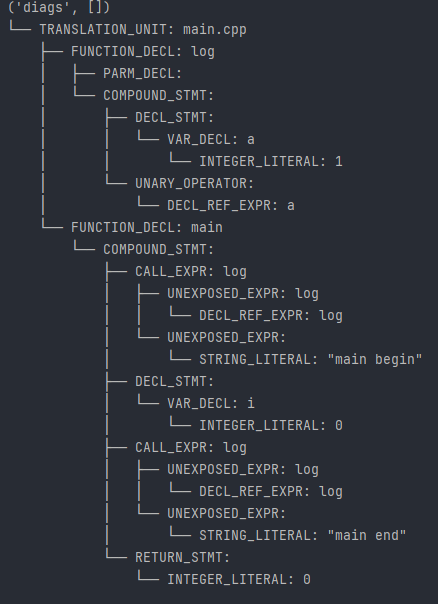
\includegraphics[width=0.5\textwidth]{pictures/AST打印.png}
	\caption{AST打印}
	\label{fig:AST打印}
\end{figure}
\subsection{解析AST,生成CFG}
不同于c++,在python中语法树的基本节点都是由Cursor组成的,我们也是通过返回Cursor的
kind类型来判断节点对应的类型。下面对于Cursor中一些比较常用的属性做出解释:
\begin{itemize}
	\item spelling:节点的名称,若节点为函数就是函数名
	\item displayname:与前者差不多,但是对于函数会多一个参数
	\item type:节点的元素类型,比如int
	\item location:节点在文件中的位置,行数,列数等
\end{itemize}
 还有一些成员方法:
\begin{itemize}
	\item get\_children:获取所有的子节点,返回一个生成器
	\item get\_tokens:获取当前节点的所有tokens,也是返回一个生成器
    \item is\_definition:判断该节点属于函数定义还是声明
\end{itemize}
{\small
\begin{lstlisting}[language=Python,caption=Graph]
class Graph:
    def __init__(self):
...
    def draw(self):
...
    def toGexf(self):
...
\end{lstlisting}
}
对于基本的图结构,本系统设计了一个Graph类,采用了networkx中的有向图来存储,并对一些常用的方法进行封装,
这样在开发时,我们便只用关心对state节点的操作,它能自动的为节点分配id。其中draw,toGexf方法是用来debug和展示阶段性成果的。
{\small
\begin{lstlisting}[language=Python,caption=StateNode]
class AstNode:
    def __init__(self, id, cfg=None, isStart=False, isEnd=False, showInSubGraph=False):
...
\end{lstlisting}
}
对于一个state,本系统采用了一个AstNode类,它包含了id和所属的自动机,在创建时自动加入Graph中,注意一般一个自动机在创建时
会生成两个AstNode,代表了它的入口和出口state。
简单的说,AstNode就是代表了CFG中的state。
                   

对于一个自动机,我们会构造出一个Cfg类,下面是它的初始化函数:
{\small
\begin{lstlisting}[language=Python,caption=init]
def __init__(self, cursor: Cursor, childs=None, breakTarget=None, continueTarget=None, returnTarget=None,
             parent=None, isCondition=False, showInSubGraph=False, isEmpty=False, label=None):

    self.cursor = cursor

    # for while switch
    self.breakTarget = breakTarget
    self.continueTarget = continueTarget
...

    G.Cnode_num += 1
    self.gid = G.Cnode_num
    self.startNode = AstNode(id=str(self.gid) + "Start", cfg=self, isStart=True)
    self.endNode = AstNode(id=str(self.gid) + "End", cfg=self, isEnd=True)
 ...
    G.cfgs.append(self)
    self.buildChildCfg()
\end{lstlisting}
}
多数情况下,当我们想要创建一个自动机(Cfg类)时,只需要传入相应的cursor即可,对于节点内会出现break,continue的(如for,while),我们还需要
设置相应的跳转位置,接着init函数会自动为我们生成两个初始state,并调用buildChildCfg,生成该节点的子节点的自动机。

递归生成自动机的方法是整个系统中的重要一环,所以下面将对并调用buildChildCfg方法详细介绍。
\\
{\small
\begin{lstlisting}[language=Python]
cursorChilds = list(self.cursor.get_children())
\end{lstlisting}
}
首先我们通过相应的方法获取目标cursor的子节点的cursor,因为后续会涉及到对整体结构的判断,我们需要将返回的生成器实例化为list,便于操作。
\\
\subsubsection{break和continue}
{\small
\begin{lstlisting}[language=Python]
if len(cursorChilds) == 0:
    # BREAK,CONTINUE
...
\end{lstlisting}
}
对于没有子节点的情况,我们先做处理,在本系统中,出现这种情况只可能是break和continue,所以我们只需将自动机适当的连接到跳转target上即可。
\\
{\small
\begin{lstlisting}[language=Python]
elif self.cursor.kind == CursorKind.RETURN_STMT:
    ...
elif self.cursor.kind == CursorKind.DECL_STMT:
    ...
elif self.cursor.kind == CursorKind.BINARY_OPERATOR:
    ...
elif self.cursor.kind == CursorKind.UNARY_OPERATOR:
    ...
\end{lstlisting}
}
以上的节点也不是我们需要处理了,它们都是简单的线性结构,所以我们只是为其添加了标签,方便展示。

\subsubsection{函数调用}
{\small
\begin{lstlisting}[language=Python]
 elif self.cursor.kind == CursorKind.CALL_EXPR:
            if self.cursor.spelling == "log":
...
            else:
...
\end{lstlisting}
}
当节点是函数调用的时候,我们需要做的是先到Graph的函数表内,查找对应函数的入口和出口,如果是一般的函数,就直接把函数连接到调用的位置。
但是对于log日志函数,我们获取函数的参数,并将其添加到graph的输入表中,最后将参数添加到边上,并做特殊处理,方便后续生成NFA,DFA,毕竟最终生成的自动机的边上,
唯一有用的便是这些参数。

c语言家族有三种控制结构:顺序,选择和循环。
\subsubsection{顺序结构}
{\small
\begin{lstlisting}[language=Python]
elif self.cursor.kind == CursorKind.COMPOUND_STMT:
    G.removeEdge(self.startNode, self.endNode)
    self.showInSubGraph = True
    bottom = self.endNode
    for c in reversed(cursorChilds):  # 反向
...
\end{lstlisting}
}
普通的顺序结构反应到AST上就是复合语句节点,对于这类节点,
它的子节点需要按照顺序连接,注意到我们在连接的时候选择了从后往前,
这是因为当复合语句中存在跳转时,我们需要正确提供target,但是如果正常地从前往后生成,便可能
出现跳转目标还未生成的情况。所以这就是反着连的好处。
\begin{figure}[htbp]
	\centering
	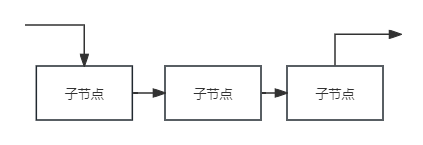
\includegraphics[width=0.5\textwidth]{pictures/顺序结构.png}
	\caption{顺序结构}
	\label{fig:顺序结构}
\end{figure}

\subsubsection{循环结构}
循环结构中,我们主要处理for和while。
{\small
\begin{lstlisting}[language=Python]
elif self.cursor.kind == CursorKind.FOR_STMT:
    l = [False, False, False]
    index = 0
    # 双指针,解析for
    tokens = self.cursor.get_tokens()
    next_token = self.cursor.get_tokens()
    next(next_token)
    for i in tokens:
...
\end{lstlisting}
}
for循环的处理比较麻烦,主要的问题是,对于for语句,三个位置(init,condition,increasement)都有可能出现空的情况,然而libclang并没有提供相关的api供我们
判断,我们也无法从语法树上简单辨认出哪个是空的,而且空的位置也会导致整个for语句执行结构发生改变。

对于这类情况,我们采用的解决方案是获取节点的token,并用";"作为判空的依据,扫描for语句的第一行,同时返回一个长度为3的list,每个位置中用布尔值表示该位置是否为空。
至于空语句导致结构改变的问题,我们直接重新设计一种专门用于空语句的节点以应对这种情况,这样我们只需要按照正常情况连接整个for语句即可。
 \begin{figure}[htbp]
	\centering
	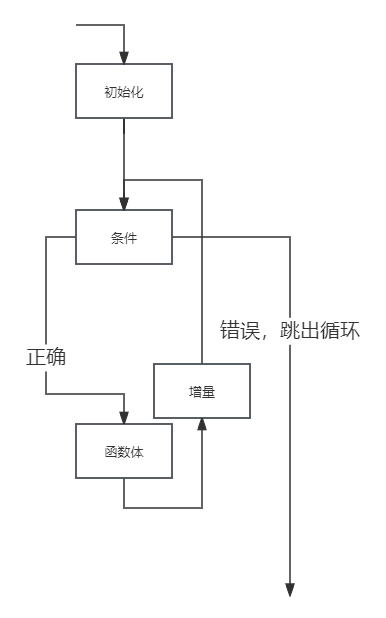
\includegraphics[width=0.5\textwidth]{pictures/for结构.png}
	\caption{for结构}
	\label{fig:for结构}
\end{figure}
{\small
\begin{lstlisting}[language=Python]
elif self.cursor.kind == CursorKind.WHILE_STMT:
    con = cursorChilds[0]
    stmts = cursorChilds[-1]
    conCfg = Cfg(con, parent=self, isCondition=True, showInSubGraph=True, label="WHILE_COND")

    # 提供breaktarget
    stmtsCfg = Cfg(stmts, breakTarget=self.endNode, continueTarget=self.startNode, parent=self,
                   showInSubGraph=True)
...
\end{lstlisting}
}
相反的,因为while语句条件必定不为空,我们只要按结构获取它的condition和body节点,依次连接即可。
 \begin{figure}[htbp]
	\centering
	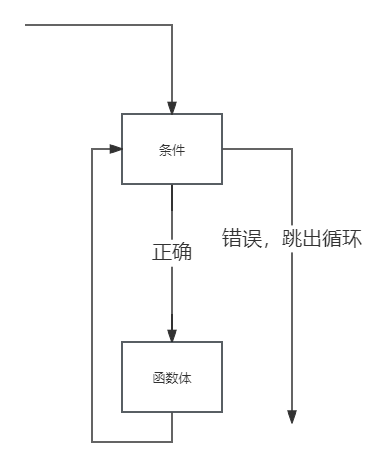
\includegraphics[width=0.5\textwidth]{pictures/while结构.png}
	\caption{while结构}
	\label{fig:while结构}
\end{figure}
\subsubsection{选择结构}
{\small
\begin{lstlisting}[language=Python]
elif self.cursor.kind == CursorKind.IF_STMT:
    con = cursorChilds[0]
    then = cursorChilds[1]
    conCfg = Cfg(con, parent=self, isCondition=True, showInSubGraph=True, label="IF_COND")
    thenCfg = Cfg(then, parent=self, continueTarget=self.continueTarget, breakTarget=self.breakTarget)
   ...
    if len(cursorChilds) > 2:
       ...
    else:
       ...
\end{lstlisting}
}
if节点中,我们需要特殊考虑子节点没有else的情况,这时条件语句错误时将
直接跳到if节点的end语句。至于if,else if等等嵌套关系,递归调用自然会帮助我们正确处理。
 \begin{figure}[htbp]
	\centering
	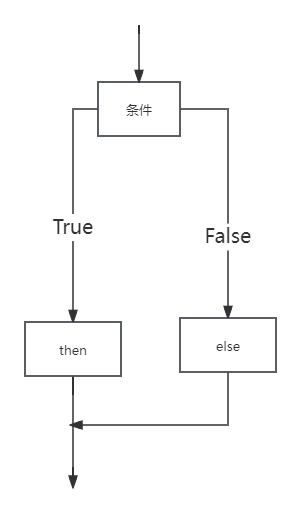
\includegraphics[width=0.3\textwidth]{pictures/if结构.png}
	\caption{if结构}
	\label{fig:if结构}
\end{figure}
{\small
\begin{lstlisting}[language=Python]
elif self.cursor.kind == CursorKind.SWITCH_STMT:
    cases = cursorChilds[-1]
    if cases.kind == CursorKind.COMPOUND_STMT:
        casesCfg = Cfg(cases, parent=self, breakTarget=self.endNode)
        ...

elif self.cursor.kind == CursorKind.CASE_STMT:
    con = cursorChilds[0]
    then = cursorChilds[1]
    conCfg = Cfg(con, parent=self, isCondition=True, showInSubGraph=True, label="CASE_COND")
    thenCfg = Cfg(then, parent=self, continueTarget=self.continueTarget, breakTarget=self.breakTarget)
    ...

elif self.cursor.kind == CursorKind.DEFAULT_STMT:
    ...
\end{lstlisting}
}
选择结构中还有一部分是switch语句节点,在语法树上,多个case被包在一个复合语句中,
但是我们并不能直接在上层处理所有的case,因为不能保证复合语句只有case节点。
所以正确的做法是把问题留给下层,单独处理每一个case。

对于单个case,它们都有类似if一样的condition和body,同样的,当条件不匹配时,
我们将直接跳转到下一条语句,但是如果成功匹配,运行完case的body后我们将
退出整个switch语句。
 \begin{figure}[htbp]
	\centering
	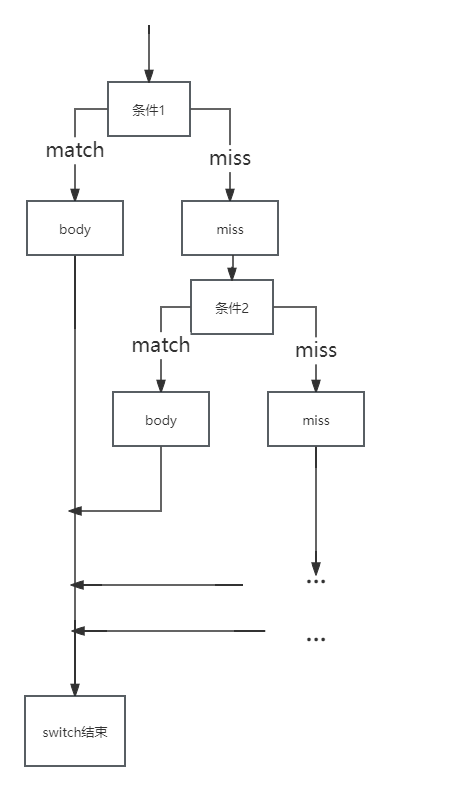
\includegraphics[width=0.5\textwidth]{pictures/switch结构.png}
	\caption{switch结构}
	\label{fig:switch结构}
\end{figure}
\subsection{从CFG生成NFA,最终生成DFA}
